\documentclass{beamer}
%
% Choose how your presentation looks.
%
% For more themes, color themes and font themes, see:
% http://deic.uab.es/~iblanes/beamer_gallery/index_by_theme.html
%
\mode<presentation>
{
  \usetheme{default}      % or try Darmstadt, Madrid, Warsaw, ...
  \usecolortheme{default} % or try albatross, beaver, crane, ...
  \usefonttheme{default}  % or try serif, structurebold, ...
  \setbeamertemplate{navigation symbols}{}
  \setbeamertemplate{caption}[numbered]
}

\usepackage{amsmath}
\usepackage[english]{babel}
\usepackage[utf8]{inputenc}
\usepackage[T1]{fontenc}
\usepackage{algorithm}
\usepackage{algorithmic}
\usepackage{subfig}
\usepackage{stackengine}


% Slide numbers
\addtobeamertemplate{navigation symbols}{}{
    \usebeamerfont{footline}
    \usebeamercolor[fg]{footline}
    \hspace{1em}
    \insertframenumber/\inserttotalframenumber
}

\setbeamertemplate{bibliography item}{\insertbiblabel}

\title[]{PalmTree: Learning an Assembly Language Model for Instruction Embedding}
\author{Xuezixiang Li, Qu Yu, Heng Yin}
\date{2021 Conference on Computer and Communications Security}

\setcounter{MaxMatrixCols}{20}


\begin{document}

\begin{frame}
  \titlepage
\end{frame}

% Uncomment these lines for an automatically generated outline.
%\begin{frame}{Outline}
%  \tableofcontents
%\end{frame}

\begin{frame}{Overview}
	
\begin{itemize}
	\item Deep learning has been successful in a variety of binary analysis tasks
	\item Important aspect of these algorithms is how to represent an instruction as a vector
	\item PalmTree is a pretrained BERT analogue that learns high-quality instruction embeddings that can be used for downstream tasks
\end{itemize}

\end{frame}

\begin{frame}{How to Feed a Neural Network}
	
	\begin{itemize}
		\item Three options: 
		\begin{enumerate}
			\item raw-byte encoding, 
			\item manual encoding of disassembled instructions, or
			\item learning-based encoding
		\end{enumerate}
		% Best option is to learn the vector representation:
			% No human efforts required (error prone and domain expertise required)
			% Can learn deeper, higher level features beyond human capabilities
	\end{itemize}

	\begin{figure}[h]
		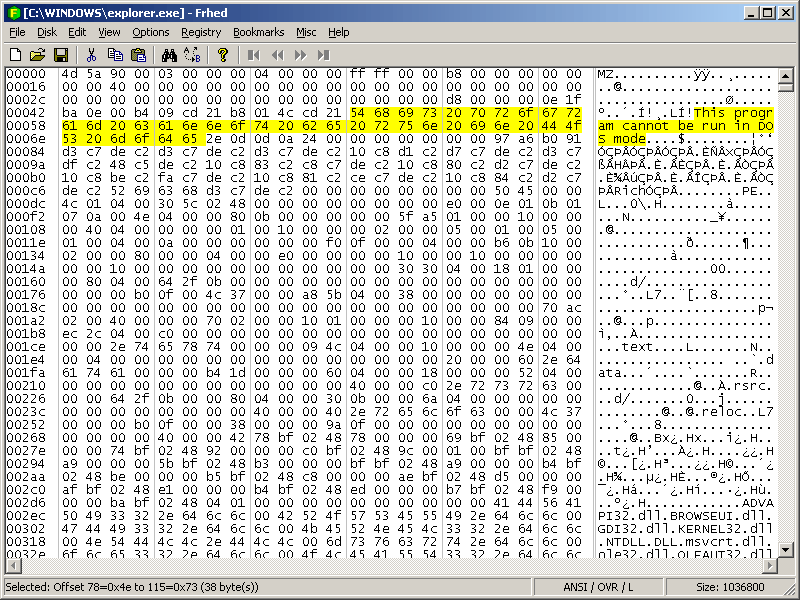
\includegraphics[scale=.25]{images/binary-hex-view.png}
	\end{figure}
	
\end{frame}

\begin{frame}{Raw-byte Encoding}
	
	\begin{itemize}
		\item One-hot encoding of bytes into a 256 dimensional vector % slight variations on this technique exist in the literature
		$$0x01 \rightarrow \begin{bmatrix} 1 & 0 & \dots & 0 \end{bmatrix}$$
		$$0xFF \rightarrow \begin{bmatrix} 0 & 0 & \dots & 1 \end{bmatrix}$$
		\item Simple, efficient, but captures no semantic information about instructions
		% Doesn't even know that 0x89 is the mov command for x86 architectures while 0xFF and 0x01 have no similar meaning
		% DNNs can probably learn some of these things on there own but it would be better to have semantic bearing representations
	\end{itemize}
	
\end{frame}

\begin{frame}{Manual Encoding of Disassembled Instructions}
	
	\begin{itemize}
		\item Binary is disassembled, different components are identified and assigned one-hot vectors, which are then concatenated
		\begin{eqnarray*}
			\textrm{mul eax, ebx} 
			&\rightarrow& \vec{\textrm{opcode}} \oplus \vec{\textrm{registers}} \oplus \vec{\textrm{addresses}} \\
			&\rightarrow& \begin{bmatrix} 0 \\ 1 \\ \vdots \\ 0 \end{bmatrix}^T \oplus \begin{bmatrix} 1 \\ 1 \\ \vdots \\ 0 \end{bmatrix}^T \oplus \begin{bmatrix} 0 \\ 0 \\ \vdots \\ 0 \end{bmatrix}^T %\\
			% &\rightarrow& \begin{bmatrix} 0 & 1 & \dots & 0 & 1 & 1  & \dots & 0 & 0 & 0 & \dots & 0 \end{bmatrix}
		\end{eqnarray*}
		\item More semantic meaning than raw-byte, but could be more
		% add \& sub have similar meanings and should be closer together in the embedding space than jz \& je
	\end{itemize}
	
\end{frame}

\begin{frame}{Learning-based Encoding}
	
	\begin{itemize}
		\item Model instructions as words and functions as documents
		\item Use word2vec model to learn word associations % unsupervised pretraining with continuous bag-of-words or skipgrams
		\begin{eqnarray*}
			\textrm{mul eax, ebx} &\rightarrow& \vec{v_1} \\
			\textrm{div ecx, edx} &\rightarrow& \vec{v_2} \\
			\textrm{jz} &\rightarrow& \vec{v_3}
		\end{eqnarray*}
		$$\textrm{distance}(\vec{v_1}, \vec{v_2}) \ll \textrm{distance}(\vec{v_1}, \vec{v_3})$$
		\item Results in semantically similar units having close vector representations, i.e., captures the most semantic meaning!
	\end{itemize}
	
\end{frame}

\begin{frame}{Challenges in Learning-based Encoding}
	
	\begin{itemize}
		\item Complex and diverse instruction formats
		% an instruction can have between 0 to 3 operands
		% an operand can be a register, a memory location, or a literal
		% implicit operands and implicit side effects, eg, EFLAGs
		\item Noisy instruction context
		% Compilers make all kinds of apparently nonsensical modifications to the source
		% NLP methods rely on the tokens immedietly before and after a particular sequence and assume they are connected.
		% Standard NLP approaches need significant adaptations
	\end{itemize}

	\begin{figure}[h]
	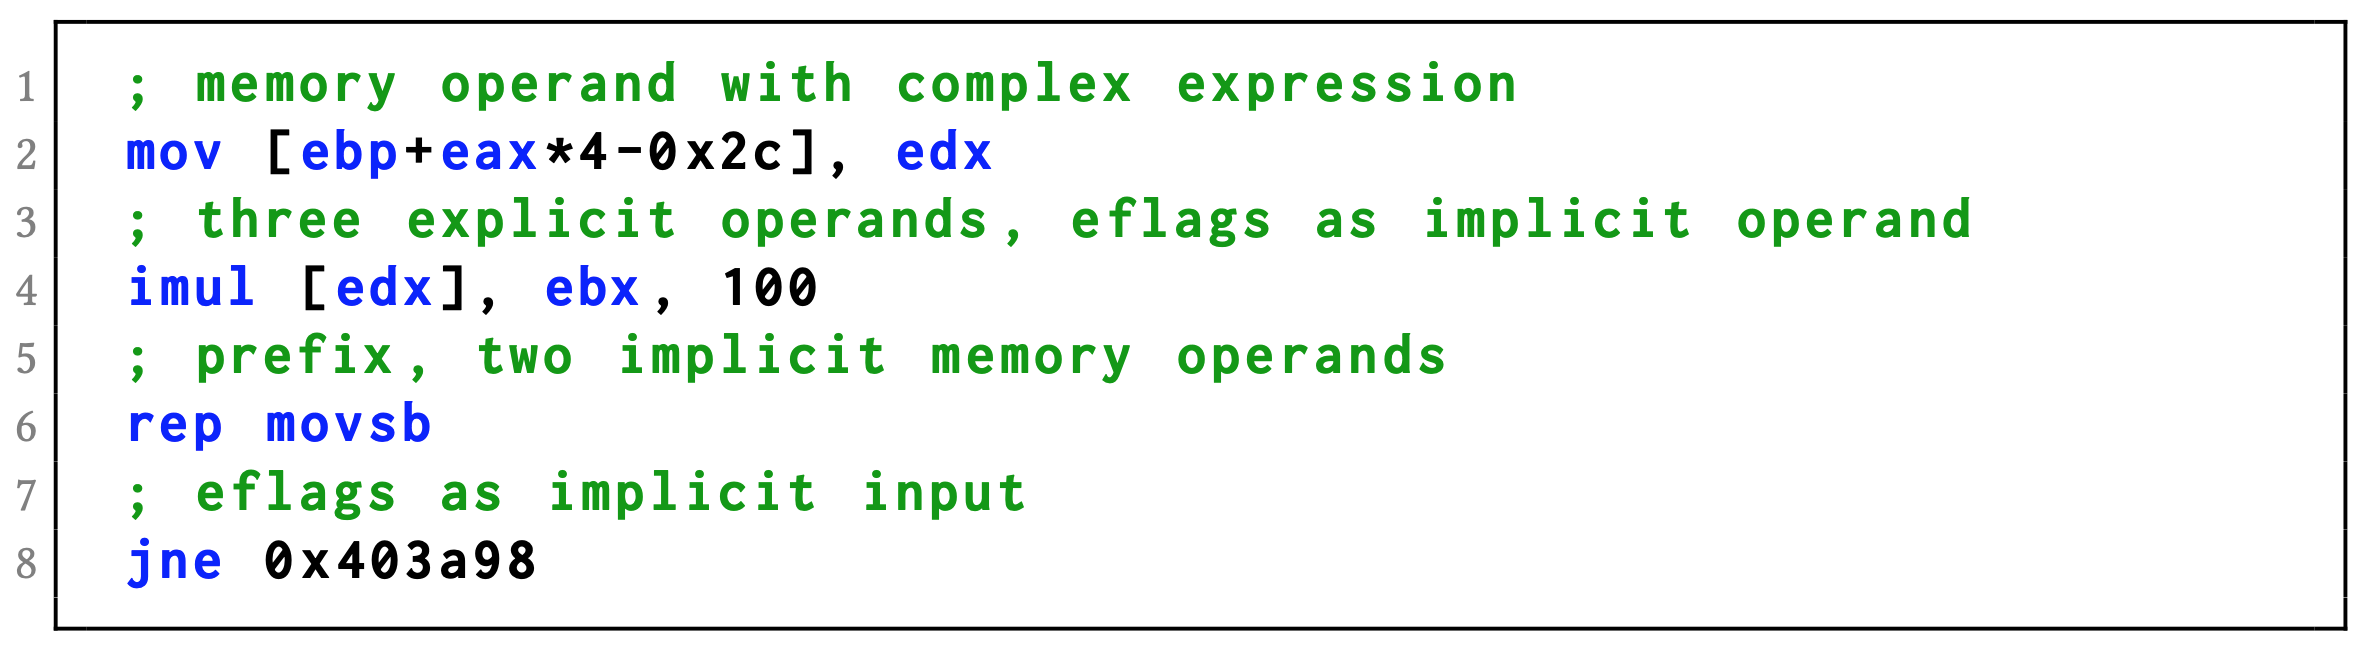
\includegraphics[scale=.25]{images/complex-diverse-instructions.png}
	\end{figure}
	
\end{frame}

\begin{frame}{PalmTree: Pre-trained Assembly Language Model for InsTRuction EmbEdding}

	\begin{figure}[h]
	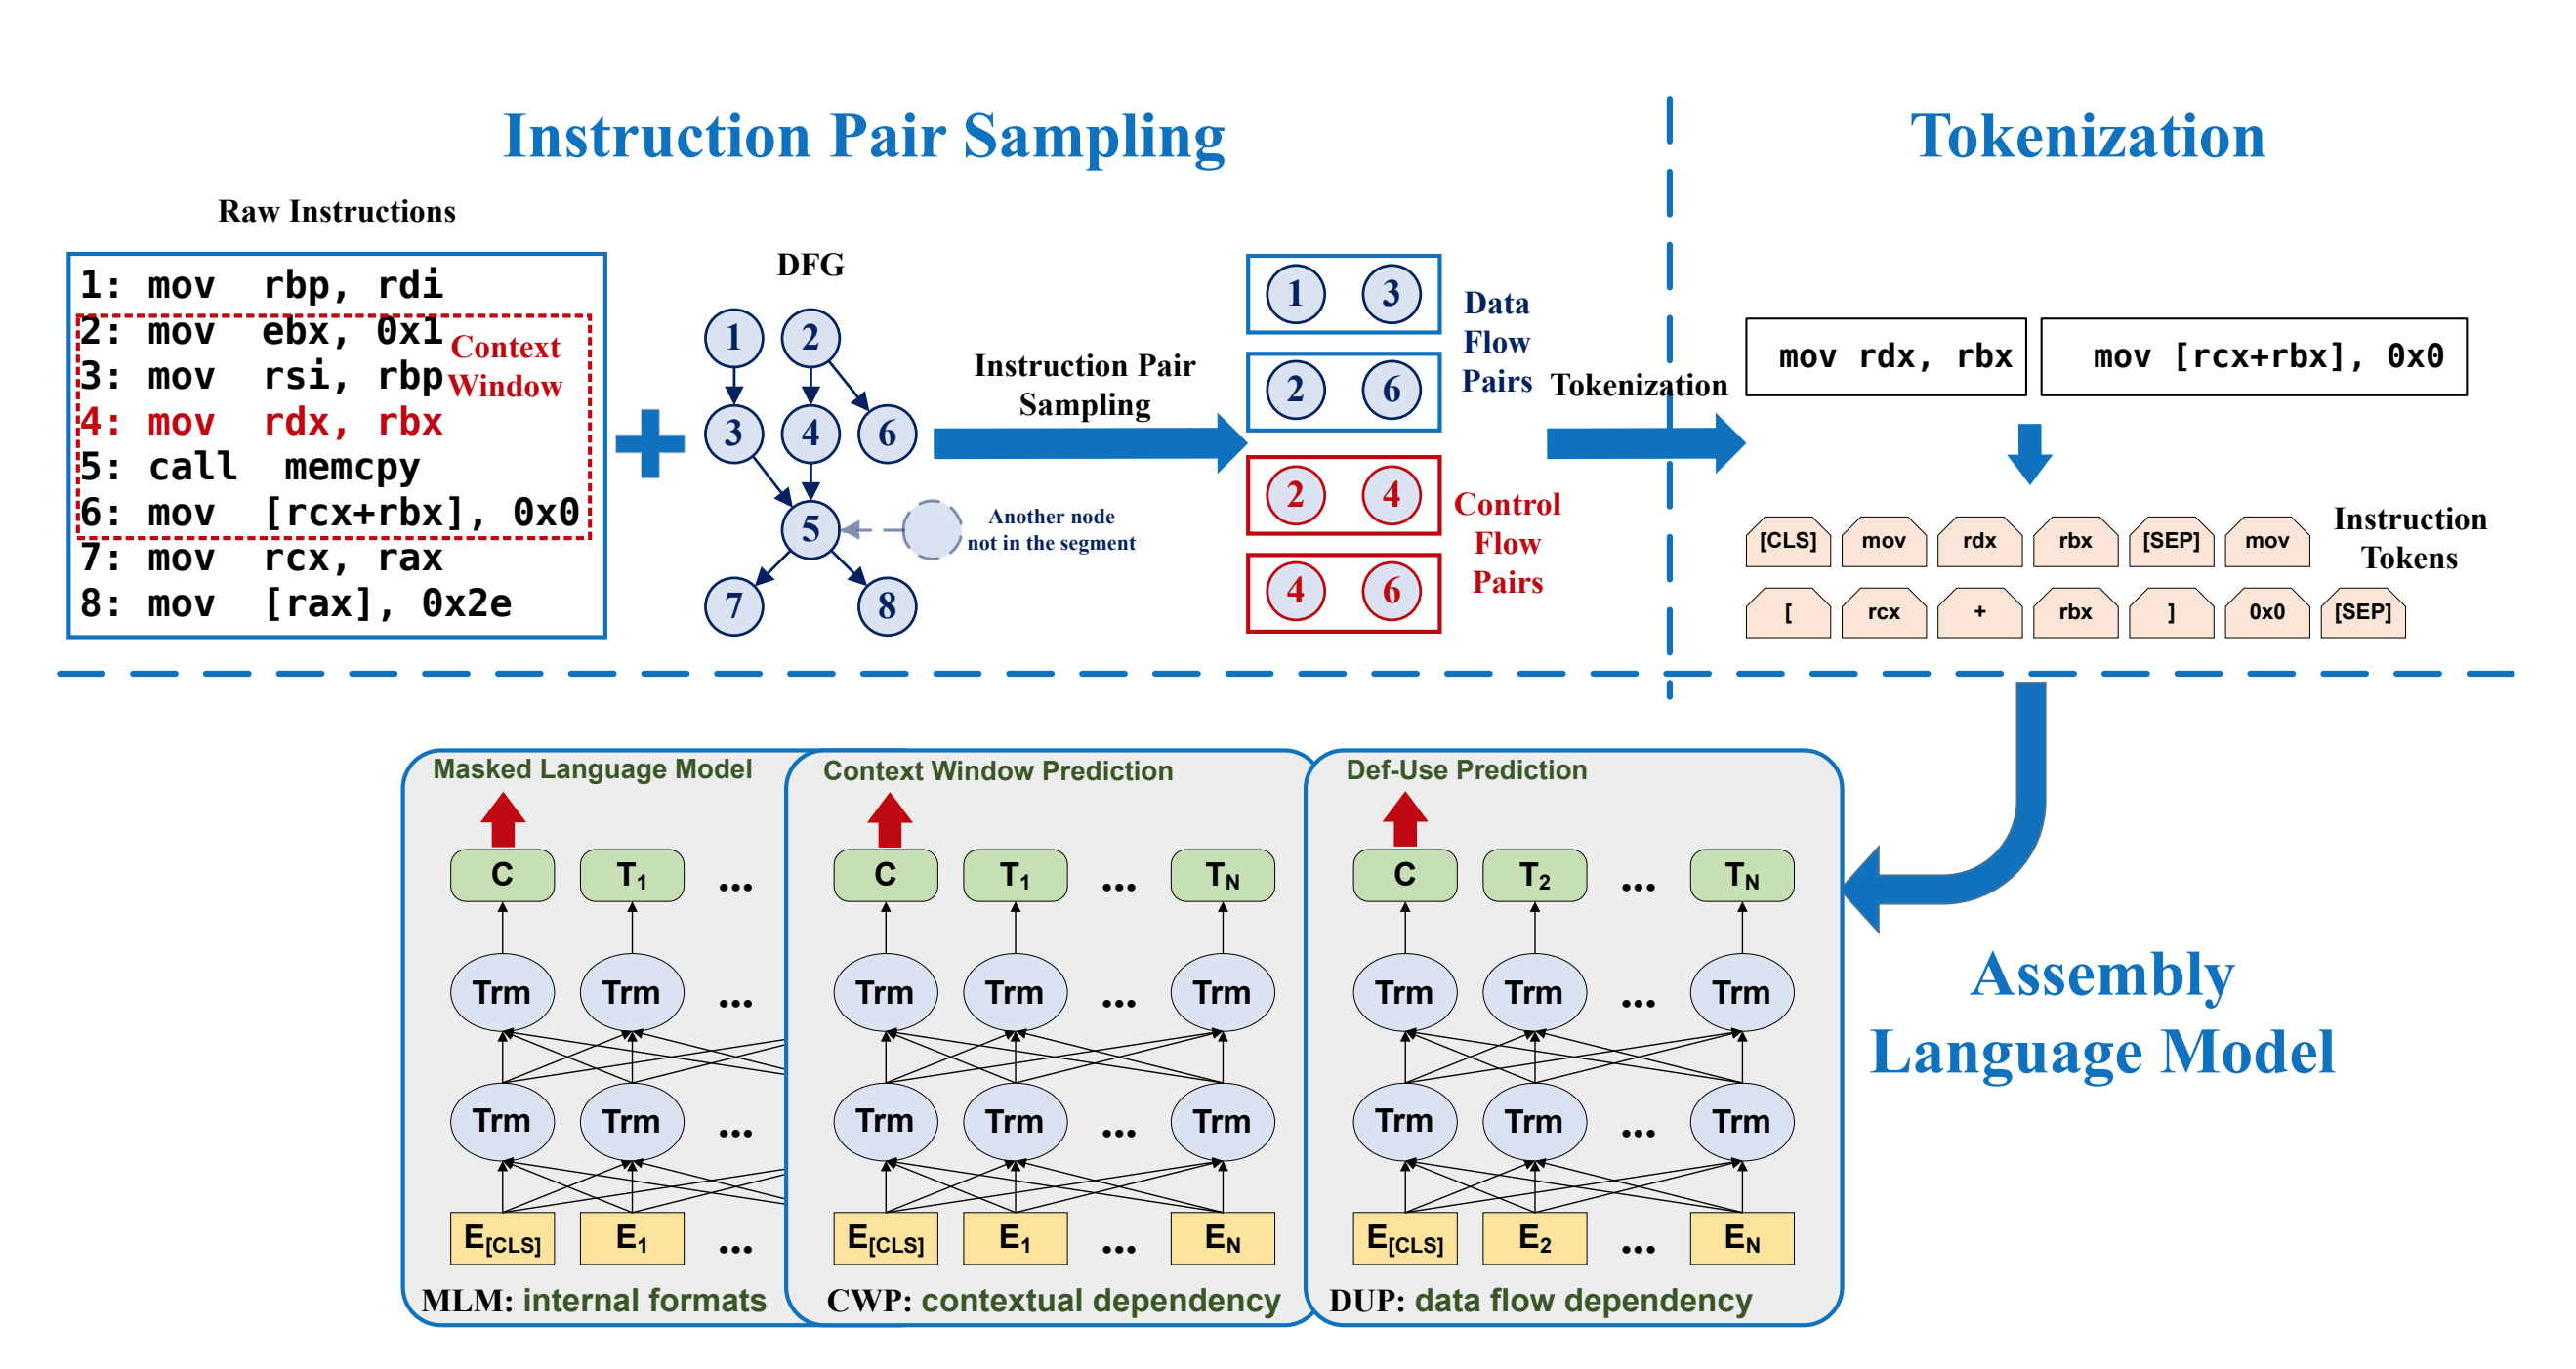
\includegraphics[scale=.225]{images/PalmTree-overview.png}
	\end{figure}
	
\end{frame}

\begin{frame}{Instruction Pair Sampling \& Tokenization}
	
	\begin{itemize}
		\item Sample instruction pairs for downstream training tasks:
		\begin{enumerate}
			\item two instructions have a \textit{def-use relation} if their is any dependency between them % registers, memory locations, function call arguments, EFLAGS
			\item two instructions have a \textit{control-flow relation} if one instruction follows the other within a certain window size
		\end{enumerate}
		\item Fine-grained instruction tokenization % vocab substitutions reduce size of vocabulary and prevent out of vocabulary errors
		\begin{enumerate}
			\item strings $\rightarrow$ `[STR]'
			\item addresses $\rightarrow$ `[ADDR]'
		\end{enumerate}
		\item Example:
		\begin{enumerate}
			\item 'mov ebx, 0x1'
			\item 'mov rdx, rbx'
		\end{enumerate}
	\end{itemize}

	\begin{figure}[h]
	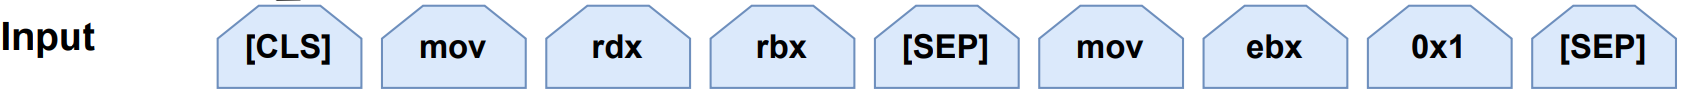
\includegraphics[scale=.35]{images/instruction-pair-sampling.png}
	\end{figure}
	
\end{frame}

\begin{frame}{Assembly Language Model: Architecture}
	
	\begin{itemize}
		\item PalmTree uses BERT (Bidirectional Encoder Representations from Transformers) architecture
	\end{itemize}

	\begin{figure}[h]
	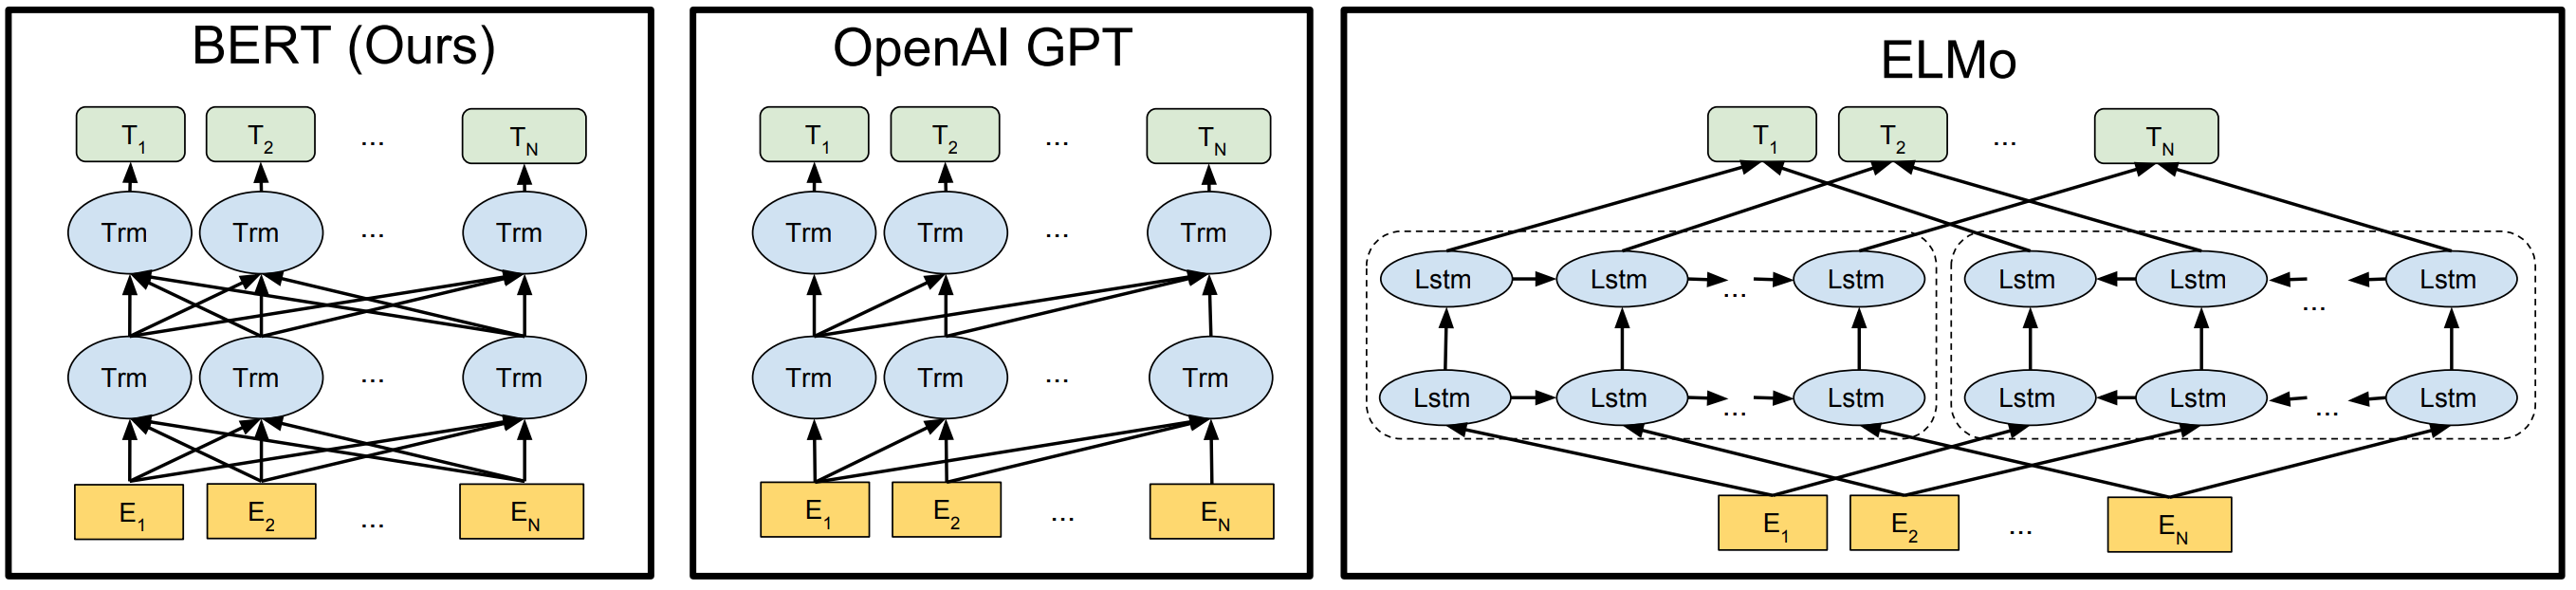
\includegraphics[scale=.225]{images/BERT-GPT-ELMo.png}
	\end{figure}
	
\end{frame}

\begin{frame}{Pretraining Task I: MLM}
	
	\begin{itemize}
		\item Masked Language Modeling (MLM) masks/corrupts a token in a sequence and tasks the model to predict the masked token
		% Allows the model to learn internal structure of instruction language
		% 15% chance to select a token; 80% chance to mask, 10% chance to corrupt, 10% chance to leave
		\item Example:
		\begin{enumerate}
			\item 'mov ebx, 0x1'
			\item 'mov rdx, rbx'
		\end{enumerate}
	\end{itemize}

	\begin{figure}[h]
	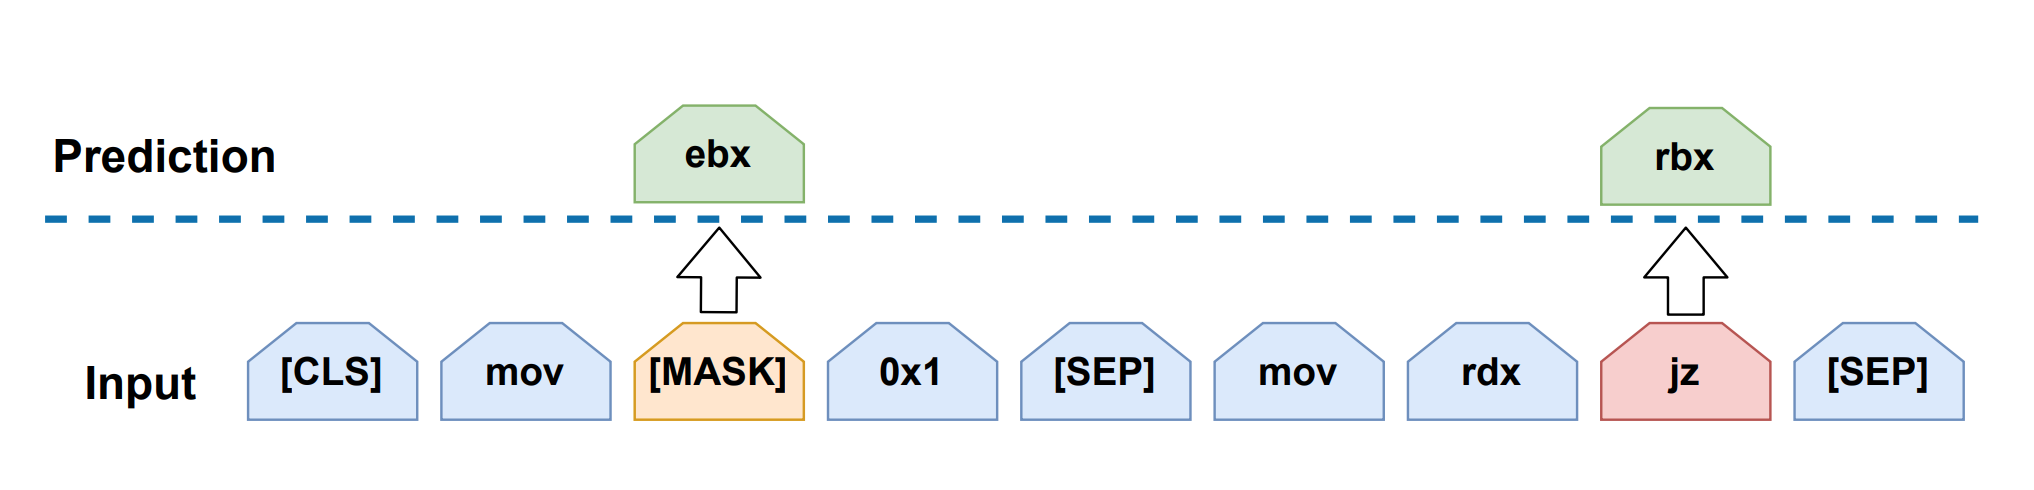
\includegraphics[scale=.3]{images/masked-language-modeling.png}
	\end{figure}
	
	% We don't need to go into the weeds on the math, but I want to demonstrate the thoroughness of this paper
	% They put a softmax layer on top of the network and use cross entropy loss over the masked tokens in a particular instruction
	$$\mathcal{L}_{\textrm{MLM}} = - \sum_{t_i \in m(I)} log{p(\hat{t} | I)}$$
	% t hat - the token prediction
	% I - instruction
	% m(I) masked tokens of the sentence
	
\end{frame}

\begin{frame}{Pretraining Task II: CWP}
	
	\begin{itemize}
		\item Context Window Prediction (CWP) predicts whether or not two instructions occur within a fixed-context window of size $w$
		% Allows the model to learn relationships between instructions
		% Context window, as opposed to NSP from BERT, gives the model robustness to compiler optimizations
		% Draws inspiration from the continuous bag of words model proposed in word2vec paper
		\item Example:
		\begin{enumerate}
			\item 'mov ebx, 0x1'
			\item 'mov rdx, rbx'
		\end{enumerate}
	\end{itemize}

	\begin{figure}[h]
	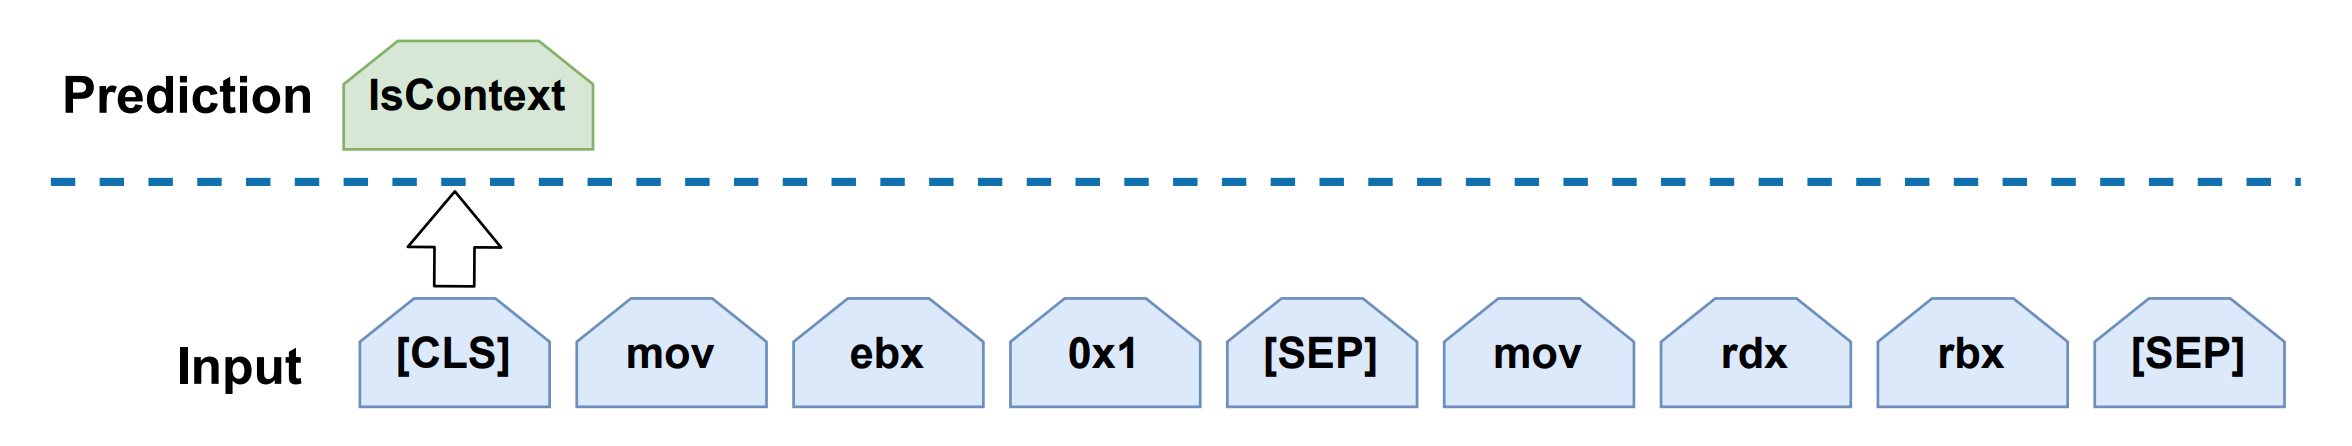
\includegraphics[scale=.25]{images/context-window-prediction.png}
	\end{figure}

	% 
	$$\mathcal{L}_{\textrm{CWP}} = - \sum_{I \in D} log{p(\hat{y} | I, I_{cand})}$$
	% D - dataset of instructions
	% 

\end{frame}

\begin{frame}{Pretraining Task III: DUP}
	
	\begin{itemize}
		\item Def Use Prediction (DUP) predicts whether or not a pair of instructions have been swapped
		% Allows the model to learn data dependencies within the instructions
		\item Example:
		\begin{enumerate}
			\item 'mov ebx, 0x1'
			\item 'mov rdx, rbx'
		\end{enumerate}
	\end{itemize}

	\begin{figure}[h]
	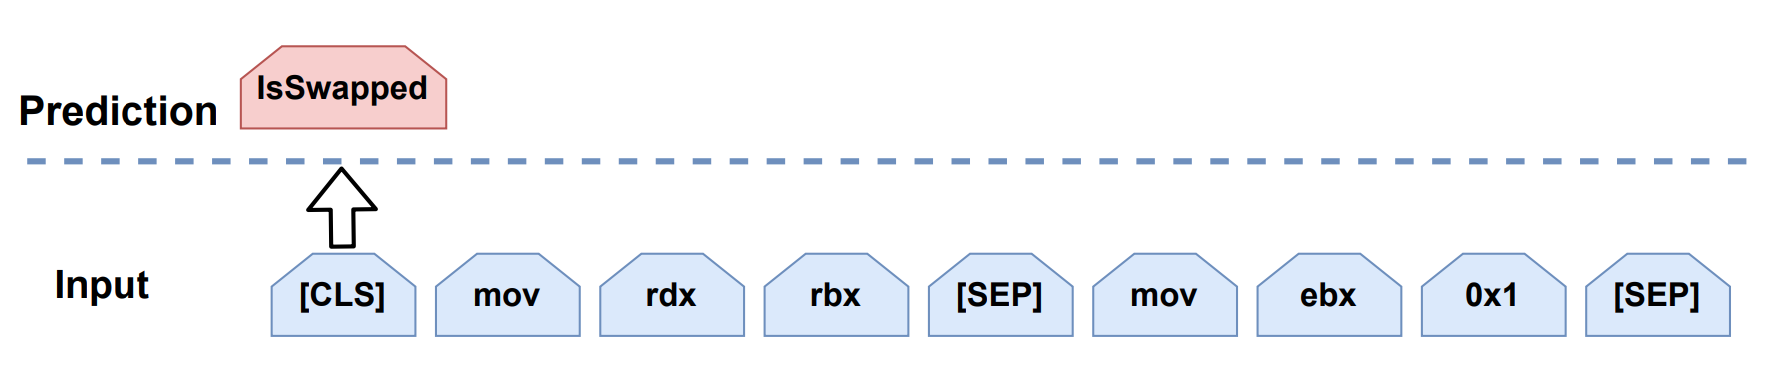
\includegraphics[scale=.3]{images/def-use-prediction.png}
	\end{figure}

	$$\mathcal{L}_{\textrm{DUP}} = - \sum_{I \in D} log{p(\hat{y} | I_1, I_2)}$$
	
\end{frame}

\begin{frame}{PalmTree Summary}
	
	\begin{itemize}
		\item Multi-task pretraining objectives give PalmTree a strong understanding of the structure, relationships, and data dependencies of assembly instructions
	\end{itemize}

	$$
	\mathcal{L_{\textrm{PalmTree}}} = \mathcal{L}_{\textrm{MLM}} + \mathcal{L}_{\textrm{CWP}} + \mathcal{L}_{\textrm{DUP}}
	$$
	
	%\begin{alignat*}{2}
	%	\mathcal{L_{\textrm{PalmTree}}} 
	%	&=  && \mathcal{L}_{\textrm{MLM}} + \mathcal{L}_{\textrm{CWP}} + \mathcal{L}_{\textrm{DUP}} \\
	%	&=  &&- \sum_{t_i \in m(I)} log{p(\hat{t} | I)} \\
	%	& &&- \sum_{I \in D} log{p(\hat{y} | I, I_{cand})} \\
	%	& &&- \sum_{I \in D} log{p(\hat{y} | I_1, I_2)}
	%\end{alignat*}

	\begin{itemize}
		\item PalmTree can be frozen an used to generate instruction embeddings or can be fine-tuned directly for downstream tasks
	\end{itemize}
	
\end{frame}

\begin{frame}{Experiment}
	
	\begin{itemize}
		\item Intrinsic Evaluation: compares different embeddings for binary analysis subtasks
		\item Extrinsic Evaluation: compares different embeddings with state-of-the-art models for downstream binary analysis tasks
		% Intrinsic evaluations aim to evaluate an NLP method on smaller, local tasks (very efficient evaluation method)
		% Extrinsic evaluations aim to evaluate the quality of an embedding scheme along with a downstream machine learning model in an end-to-end manner
		\item PalmTree variants:
		\begin{enumerate}
			\item PalmTree-M: only MLM
			\item PalmTree-MC: MLM \& CWP
			\item PalmTree: MLM, CWP, \& DUP
		\end{enumerate}
	\end{itemize}
	
\end{frame}

\begin{frame}{Intrinsic I: Outlier Evaluation}
	
	\begin{itemize}
		\item Identify the ``outlier'' instruction from a set of instructions
		% Randomly create a set of instructions, one of which is an outlier
		% Use cosine distance between embeddings to identify the outlier
		% Compare to ground truth
	\end{itemize}
	
	% Categorize x86 instructions into 12 types based upon opcode
	% Create sets of five instructions: 4 of which use opcodes belonging to the same set, 1 belongs to different set
	\begin{figure}[h]
	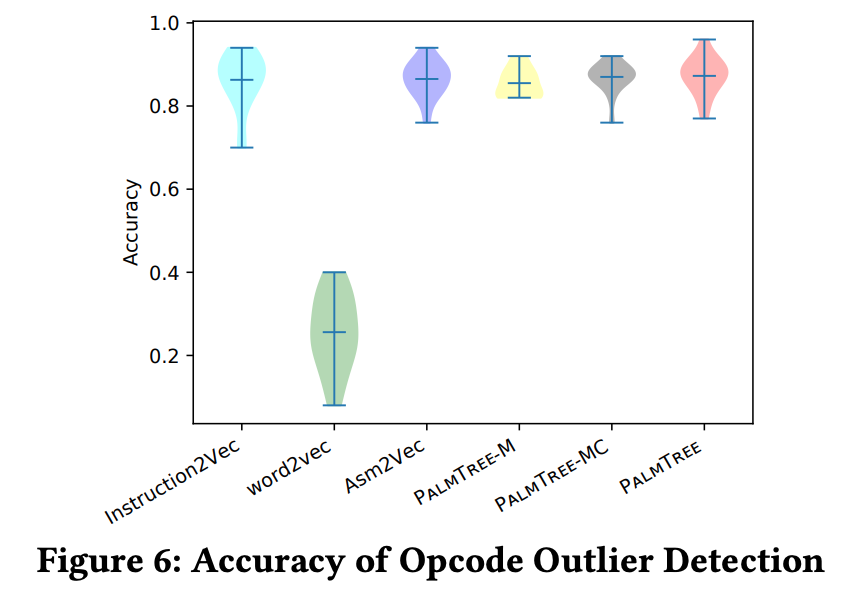
\includegraphics[scale=.3]{images/outlier-detection-opcode.png}
	\end{figure}
	
	% Similar procedure for the operand detection, except only 10 categories exist
	\begin{figure}[h]
		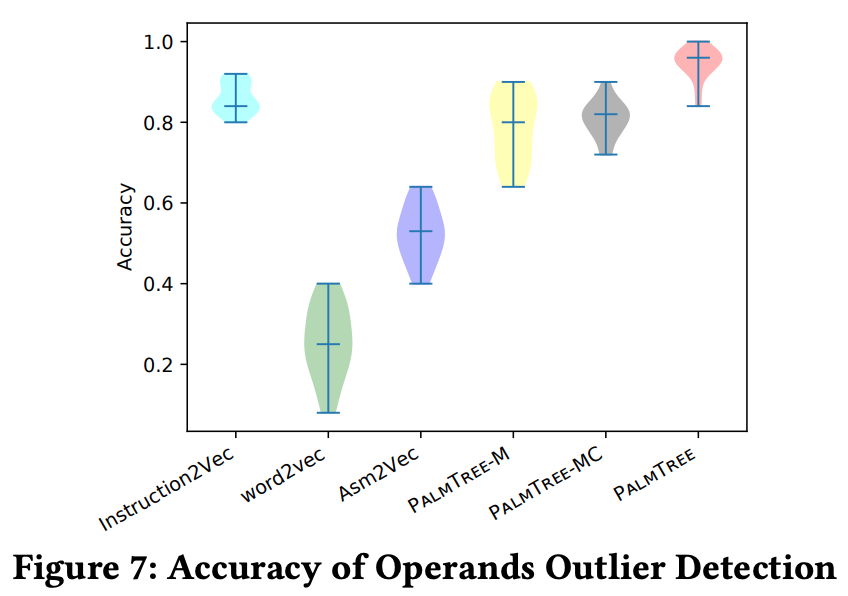
\includegraphics[scale=.3]{images/outlier-detection-operand.png}
	\end{figure}
	
\end{frame}

\begin{frame}{Intrinsic II: Basic Block Search}
	
	\begin{itemize}
		\item Find semantically equivalent blocks of x86 code
		% Compute an embedding for an entire block by averaging the embeddings for its constituent instructions
		% Find semanticaly equivalent blocks using cosine distance
		% Use ground truth from open source datasets not included in training
	\end{itemize}
	
	\begin{figure}[h]
		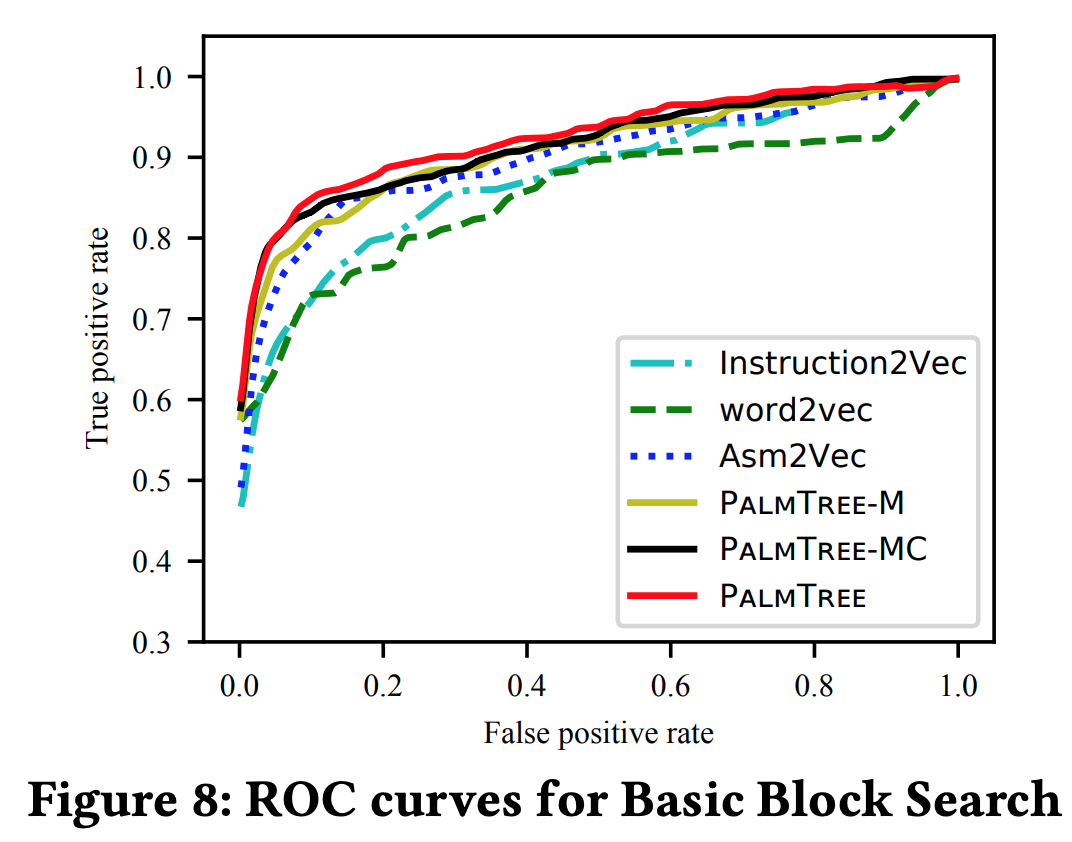
\includegraphics[scale=.3]{images/basic-block-search.png}
	\end{figure}
	
\end{frame}

\begin{frame}{Extrinsic I: Binary Code Similarity Detection}
	
	\begin{itemize}
		\item Determine if binary code is similar without access to source code
	\end{itemize}

	\begin{figure}[h]
	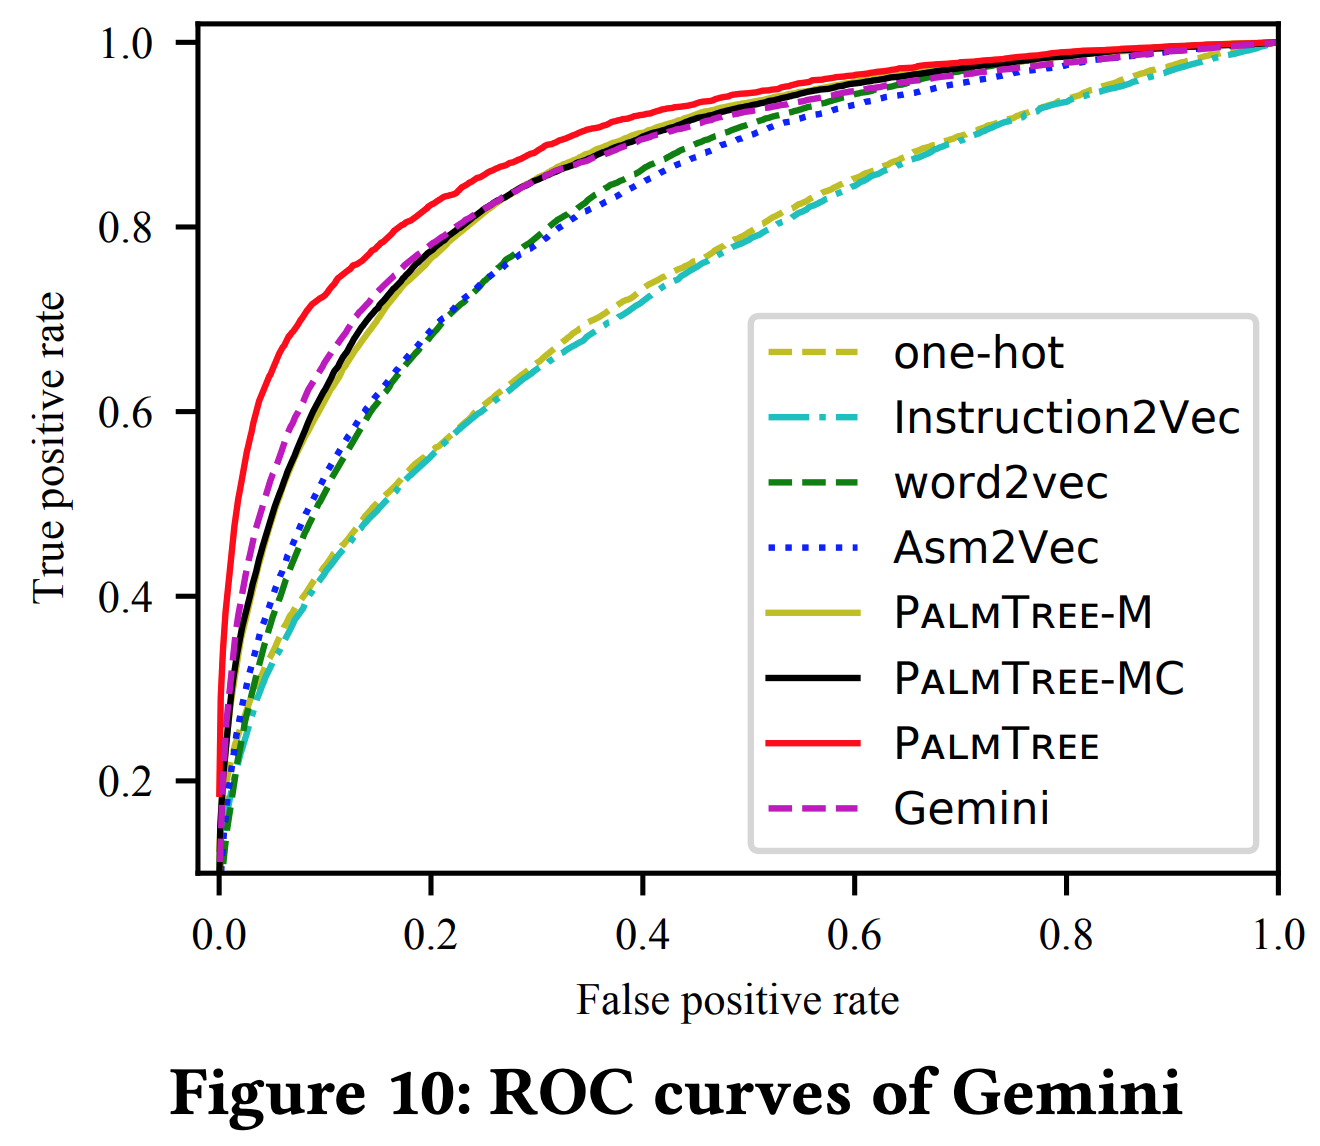
\includegraphics[scale=.3]{images/Gemini.png}
	\end{figure}
	
\end{frame}

\begin{frame}{Extrinsic II: Function Type Signature Analysis}
	
	\begin{itemize}
		\item Determine the types of function parameters and return values
	\end{itemize}

	\begin{figure}[h]
	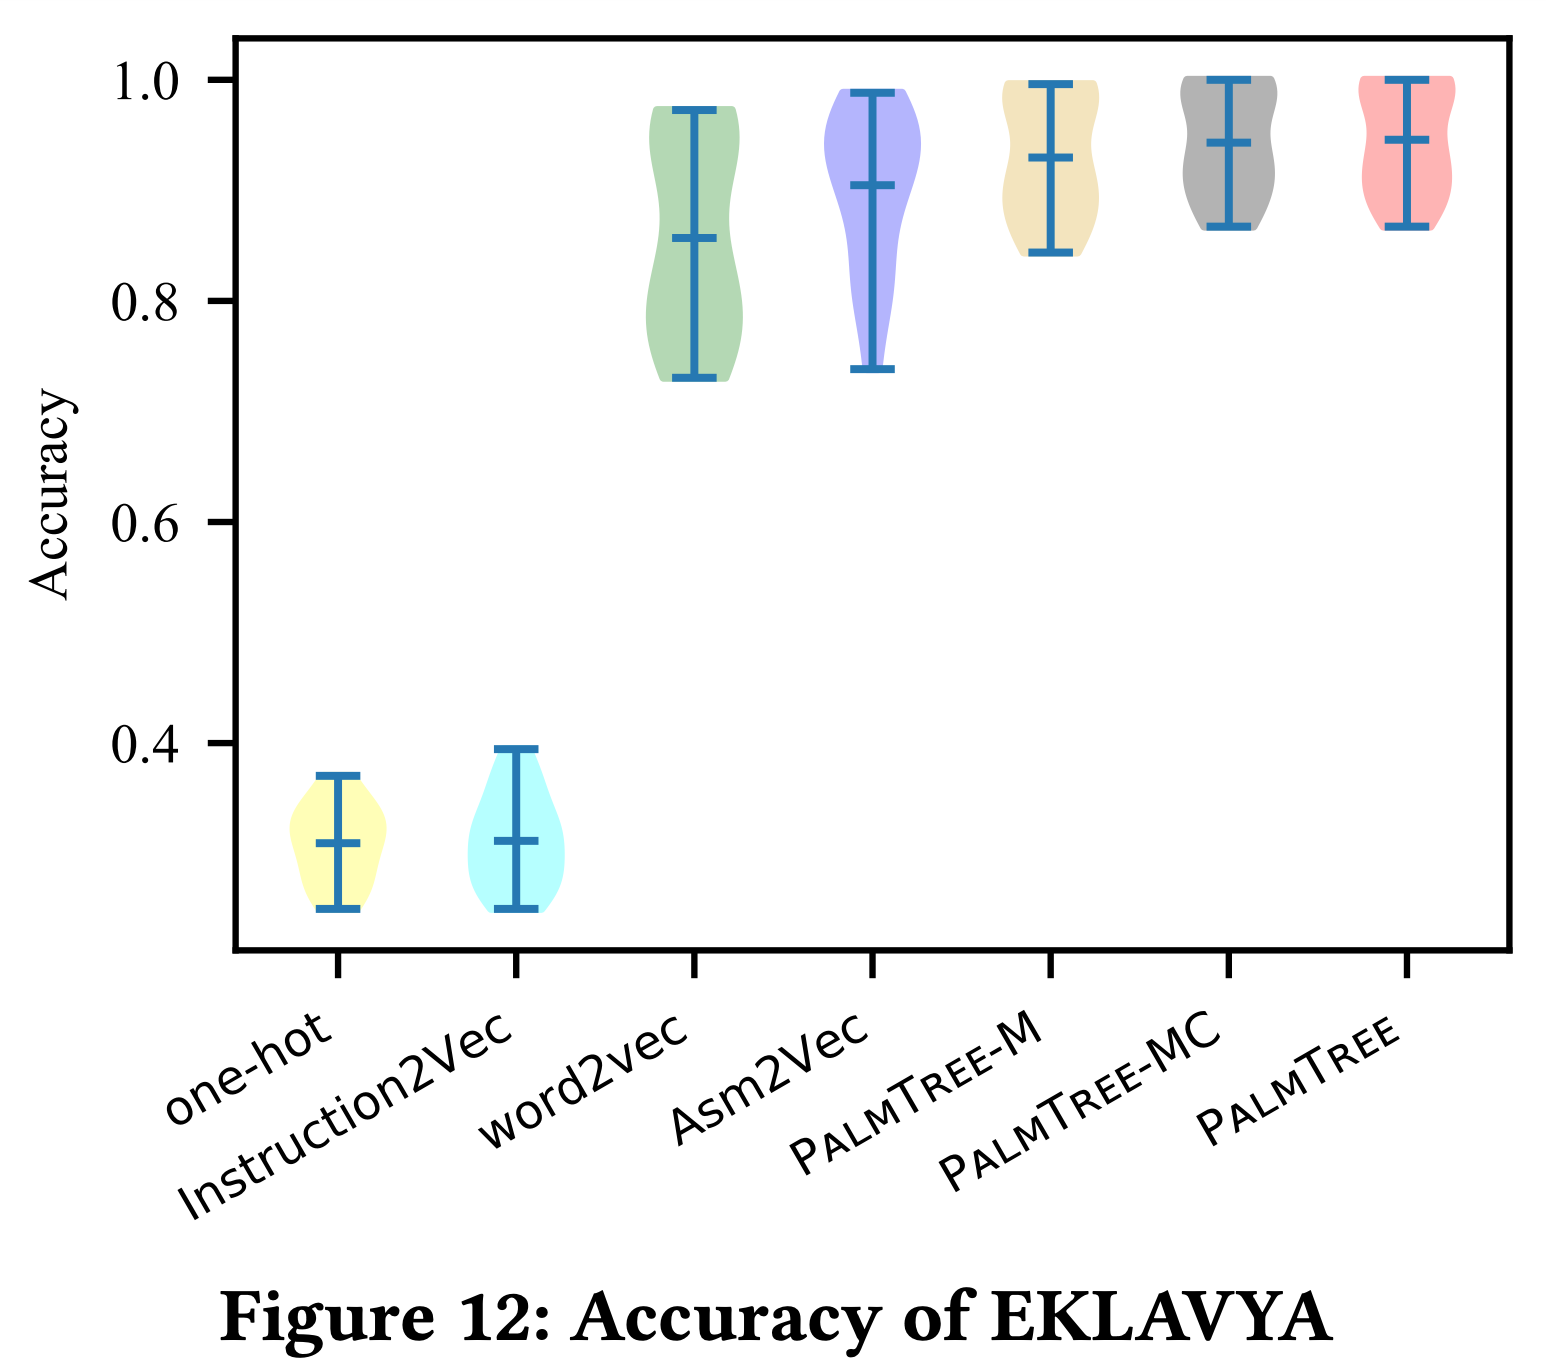
\includegraphics[scale=.3]{images/EKLAVYA.png}
	\end{figure}
	
\end{frame}

\begin{frame}{Extrinsic III: Value Set Analysis}
	
	\begin{itemize}
		\item Determine if binary code contains a memory leak
	\end{itemize}

	\begin{figure}[h]
	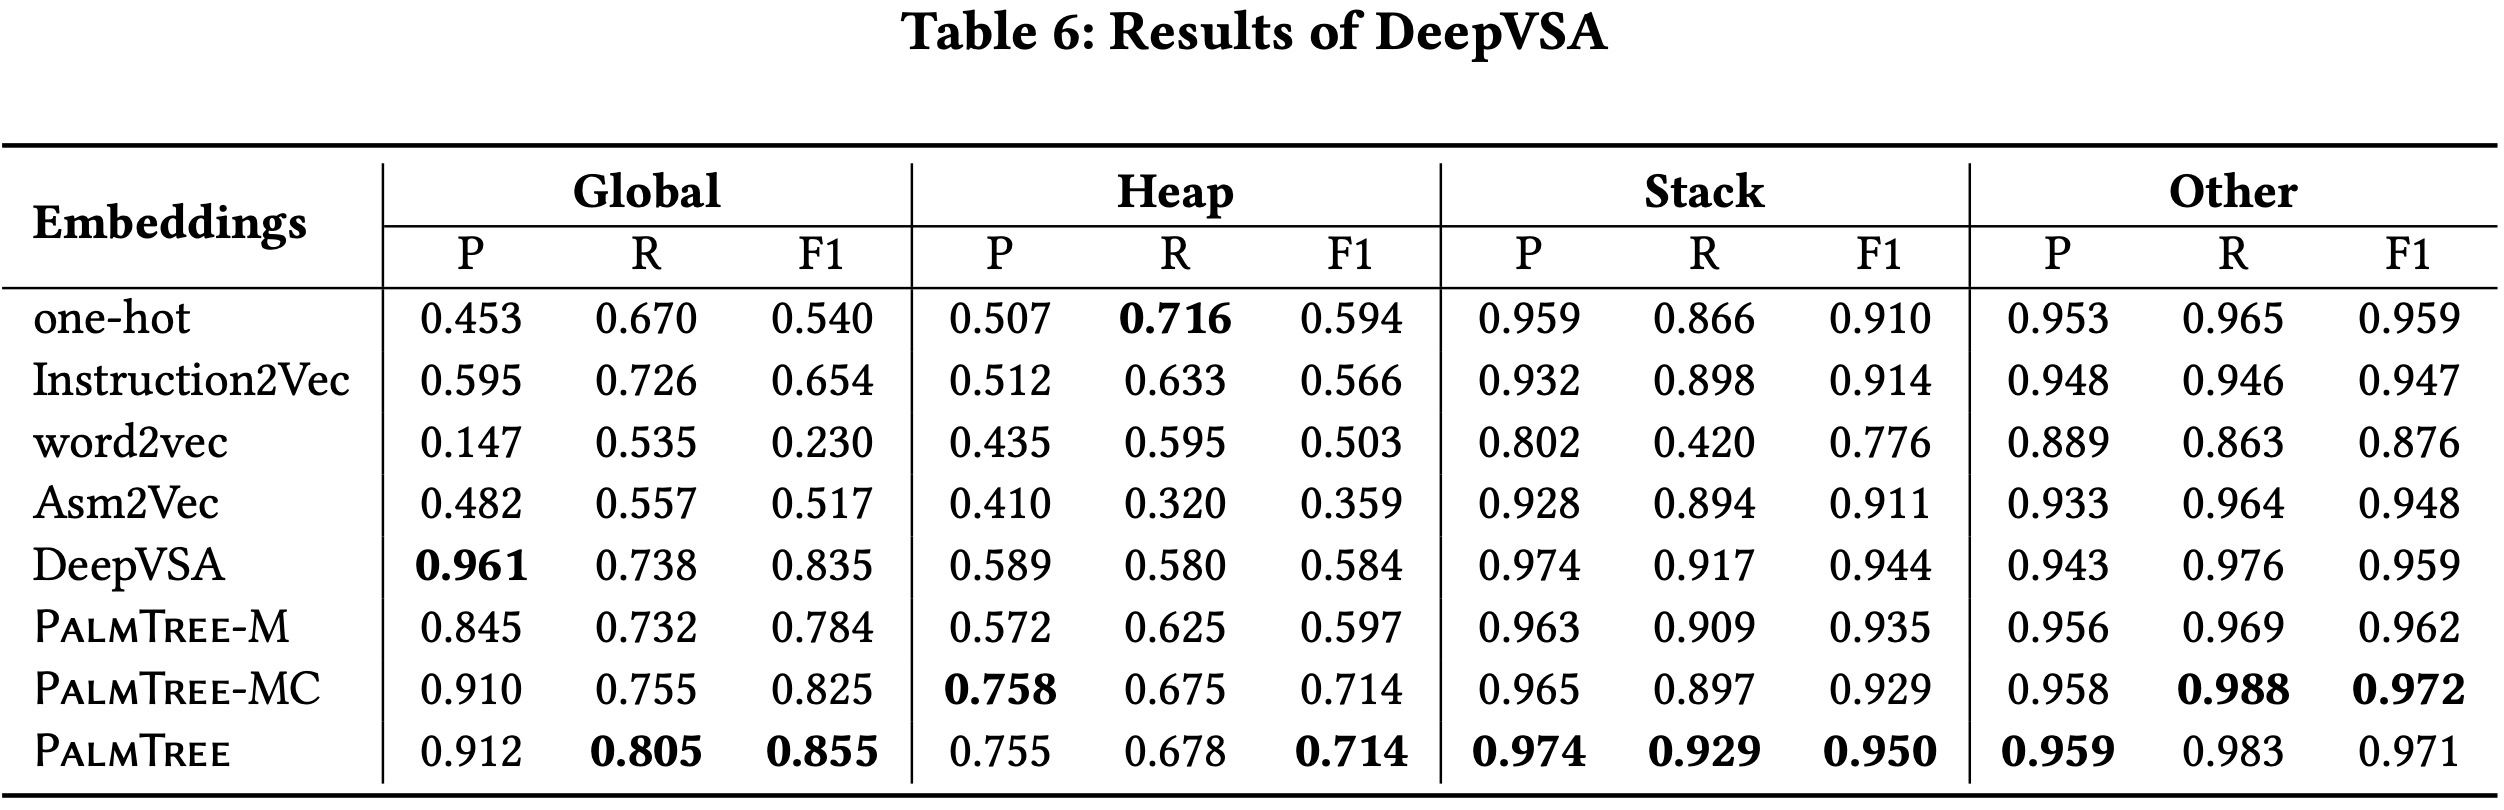
\includegraphics[scale=.225]{images/DeepVSA.png}
	\end{figure}
	
\end{frame}

\begin{frame}{Runtime Efficiency}
	
	\begin{itemize}
		\item PalmTree takes significantly longer to train and produces embeddings at a slower rate
	\end{itemize}
	
	\begin{figure}[h]
	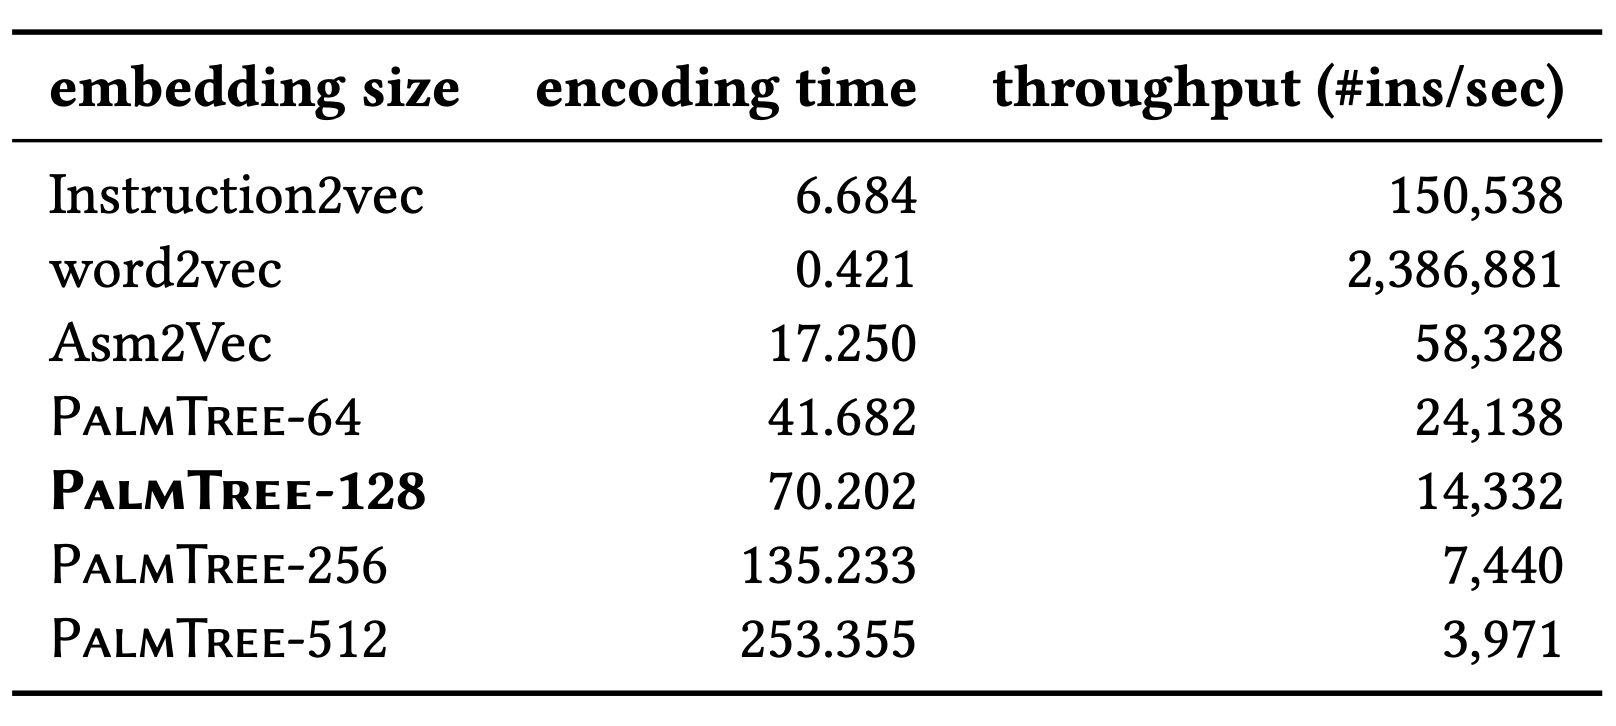
\includegraphics[scale=.3]{images/runtime-efficiency.png}
	\end{figure}

\end{frame}

\begin{frame}{Conclusions \& Future Work}
	
	\begin{itemize}
		\item PalmTree is a task-agnostic pretrained large language model for x86 instructions that can be used to train high performing binary analysis models
		\item Directions for future work include cross-architecture language modeling and improving how PalmTree handles long-range dependencies within code % feeding model more than two instructions at a time
	\end{itemize}
	
\end{frame}

\end{document}